\documentclass[a4paper,12pt]{article}
\usepackage[utf8]{inputenc}
\usepackage[danish]{babel}
\usepackage{amsmath}
\usepackage{amssymb}
\usepackage{geometry}
\usepackage{fancyhdr}
\usepackage{enumitem}
\usepackage{xcolor}
\usepackage{tcolorbox}

\geometry{margin=2.5cm}
\pagestyle{fancy}
\fancyhf{}
\rhead{Differentialligninger}
\lhead{Løsninger}
\cfoot{\thepage}

\title{\textbf{Løsninger til Opgaver om Differentialligninger}}
\author{}
\date{}

\begin{document}

\maketitle

\section*{Opgave 5}

\subsection*{Opgavebeskrivelse}
En funktion $f$ er løsning til differentialligningen
\[
\frac{dy}{dx} = 2x^2 + x + \frac{y}{x}
\]

\subsection*{a) Bestem en ligning for tangenten til grafen for $f$ i punktet $P(3,12)$}

\textbf{Løsning:}

For at finde tangentens ligning skal vi bruge:
\begin{itemize}
    \item Punktet $P(3,12)$
    \item Hældningen i dette punkt
\end{itemize}

Hældningen findes ved at indsætte $x = 3$ og $y = 12$ i differentialligningen:
\begin{align*}
\frac{dy}{dx}\bigg|_{(3,12)} &= 2 \cdot 3^2 + 3 + \frac{12}{3} \\
&= 2 \cdot 9 + 3 + 4 \\
&= 18 + 3 + 4 \\
&= 25
\end{align*}

Tangentens ligning er givet ved:
\[
y - y_1 = m(x - x_1)
\]

Hvor $(x_1, y_1) = (3, 12)$ og $m = 25$.

\begin{align*}
y - 12 &= 25(x - 3) \\
y - 12 &= 25x - 75 \\
y &= 25x - 63
\end{align*}

\textcolor{blue}{\textbf{Svar:} Tangentens ligning er $y = 25x - 63$}

\subsection*{b) Undersøg, om funktionen $g(x) = x^3 + x^2 + 5x$ er en løsning til differentialligningen}

\textbf{Løsning:}

For at $g(x)$ skal være en løsning, skal $g'(x)$ opfylde differentialligningen, dvs.:
\[
g'(x) = 2x^2 + x + \frac{g(x)}{x}
\]

Først beregner vi $g'(x)$:
\begin{align*}
g(x) &= x^3 + x^2 + 5x \\
g'(x) &= 3x^2 + 2x + 5
\end{align*}

Nu beregner vi højresiden af differentialligningen:
\begin{align*}
2x^2 + x + \frac{g(x)}{x} &= 2x^2 + x + \frac{x^3 + x^2 + 5x}{x} \\
&= 2x^2 + x + \frac{x^3}{x} + \frac{x^2}{x} + \frac{5x}{x} \\
&= 2x^2 + x + x^2 + x + 5 \\
&= 3x^2 + 2x + 5
\end{align*}

Vi ser at:
\[
g'(x) = 3x^2 + 2x + 5 = 2x^2 + x + \frac{g(x)}{x}
\]

\textcolor{blue}{\textbf{Svar:} Ja, $g(x) = x^3 + x^2 + 5x$ er en løsning til differentialligningen.}

\newpage

\section*{Opgave 4 (første version)}

\subsection*{Opgavebeskrivelse}
En funktion $f$ er bestemt ved
\[
f(x) = e^{2x} + x^2
\]

\subsection*{a) Undersøg, om $f$ er en løsning til differentialligningen $y' = 2(y + x - x^2)$}

\textbf{Løsning:}

For at undersøge om $f$ er en løsning, skal vi verificere at $f'(x) = 2(f(x) + x - x^2)$.

Først beregner vi $f'(x)$:
\begin{align*}
f(x) &= e^{2x} + x^2 \\
f'(x) &= 2e^{2x} + 2x
\end{align*}

Nu beregner vi højresiden af differentialligningen:
\begin{align*}
2(f(x) + x - x^2) &= 2(e^{2x} + x^2 + x - x^2) \\
&= 2(e^{2x} + x) \\
&= 2e^{2x} + 2x
\end{align*}

Vi ser at:
\[
f'(x) = 2e^{2x} + 2x = 2(f(x) + x - x^2)
\]

\textcolor{blue}{\textbf{Svar:} Ja, $f(x) = e^{2x} + x^2$ er en løsning til differentialligningen $y' = 2(y + x - x^2)$.}

\newpage

\section*{Opgave 4 (anden version)}

\subsection*{Opgavebeskrivelse}
En funktion $f$ er løsning til differentialligningen
\[
y' = x - y + 5
\]

Det oplyses, at grafen for $f$ går gennem punktet $P(1, 10)$.

\subsection*{a) Bestem en ligning for tangenten til grafen for $f$ i punktet $P$}

\textbf{Løsning:}

For at finde tangentens ligning skal vi bruge:
\begin{itemize}
    \item Punktet $P(1, 10)$
    \item Hældningen i dette punkt
\end{itemize}

Hældningen findes ved at indsætte $x = 1$ og $y = 10$ i differentialligningen:
\begin{align*}
y'(1) &= 1 - 10 + 5 \\
&= -4
\end{align*}

Tangentens ligning er:
\begin{align*}
y - 10 &= -4(x - 1) \\
y - 10 &= -4x + 4 \\
y &= -4x + 14
\end{align*}

\textcolor{blue}{\textbf{Svar:} Tangentens ligning er $y = -4x + 14$}

\newpage

\section*{Opgave 7}

\subsection*{Opgavebeskrivelse}
Figuren viser et hældningsfelt for en differentialligning på formen $y' = k \cdot y$.

Funktionerne $f$, $g$ og $h$ er givet ved:
\begin{align*}
f(x) &= e^{-0.5x} \\
g(x) &= 4e^{-0.5x} \\
h(x) &= 4e^{0.5x}
\end{align*}

\subsection*{a) Argumentér for, hvilken af funktionerne $f$, $g$ og $h$, der ikke kan være en løsning til differentialligningen}

\textbf{Løsning:}

For en differentialligning på formen $y' = k \cdot y$ skal forholdet $\frac{y'}{y}$ være konstant og lig med $k$.

Lad os undersøge hver funktion:

\textbf{For $f(x) = e^{-0.5x}$:}
\begin{align*}
f'(x) &= -0.5 \cdot e^{-0.5x} \\
\frac{f'(x)}{f(x)} &= \frac{-0.5 \cdot e^{-0.5x}}{e^{-0.5x}} = -0.5
\end{align*}
Så $f$ opfylder $y' = -0.5 \cdot y$ med $k = -0.5$.

\textbf{For $g(x) = 4e^{-0.5x}$:}
\begin{align*}
g'(x) &= 4 \cdot (-0.5) \cdot e^{-0.5x} = -2e^{-0.5x} \\
\frac{g'(x)}{g(x)} &= \frac{-2e^{-0.5x}}{4e^{-0.5x}} = -0.5
\end{align*}
Så $g$ opfylder også $y' = -0.5 \cdot y$ med $k = -0.5$.

\textbf{For $h(x) = 4e^{0.5x}$:}
\begin{align*}
h'(x) &= 4 \cdot 0.5 \cdot e^{0.5x} = 2e^{0.5x} \\
\frac{h'(x)}{h(x)} &= \frac{2e^{0.5x}}{4e^{0.5x}} = 0.5
\end{align*}
Så $h$ opfylder $y' = 0.5 \cdot y$ med $k = 0.5$.

\textbf{Analyse af hældningsfeltet:}

For differentialligningen $y' = k \cdot y$ afhænger hældningens fortegn af både $k$ og $y$:

\textbf{Hvis $k < 0$ (negativ):}
\begin{itemize}
    \item Når $y > 0$: $y' = k \cdot y = (\text{negativ}) \times (\text{positiv}) = \text{negativ}$ 
    
    → hældningen er negativ (kurven falder)
    \item Når $y < 0$: $y' = k \cdot y = (\text{negativ}) \times (\text{negativ}) = \text{positiv}$
    
    → hældningen er positiv (kurven stiger)
\end{itemize}

\textbf{Hvis $k > 0$ (positiv):}
\begin{itemize}
    \item Når $y > 0$: $y' = k \cdot y = (\text{positiv}) \times (\text{positiv}) = \text{positiv}$
    
    → hældningen er positiv (kurven stiger)
    \item Når $y < 0$: $y' = k \cdot y = (\text{positiv}) \times (\text{negativ}) = \text{negativ}$
    
    → hældningen er negativ (kurven falder)
\end{itemize}

\textbf{Observation fra figuren:}

Fra hældningsfeltet i opgaven kan vi se:
\begin{itemize}
    \item Over $x$-aksen ($y > 0$): Pilene peger nedad til højre → \textbf{negativ hældning}
    \item Under $x$-aksen ($y < 0$): Pilene peger opad til højre → \textbf{positiv hældning}
\end{itemize}

Dette mønster matcher situationen hvor $k < 0$.

\textbf{Konklusion:}

Siden:
\begin{itemize}
    \item $f(x) = e^{-0.5x}$ har $k = -0.5 < 0$ 
    \item $g(x) = 4e^{-0.5x}$ har $k = -0.5 < 0$ 
    \item $h(x) = 4e^{0.5x}$ har $k = 0.5 > 0$ 
\end{itemize}

\textcolor{blue}{\textbf{Svar:} Funktionen $h(x) = 4e^{0.5x}$ kan ikke være en løsning til differentialligningen, fordi den har $k = 0.5 > 0$. Dette ville give positive hældninger når $y > 0$, men hældningsfeltet viser negative hældninger når $y > 0$, hvilket indikerer at $k < 0$.}

\section{Opgave 10: Vektorfunktion}

Givet vektorfunktionen:
\[
\vec{s}(t) = \begin{pmatrix} \frac{1}{4}t^4 + 2t \\ t^3 - t + 2 \end{pmatrix}
\]

Eller skrevet som:
\begin{align*}
x(t) &= \frac{1}{4}t^4 + 2t \\
y(t) &= t^3 - t + 2
\end{align*}

\section{Forskellige typer tangenter}

\subsection{1. Vandret tangent (allerede fundet)}

En \textbf{vandret tangent} opstår når $\frac{dy}{dt} = 0$ (mens $\frac{dx}{dt} \neq 0$).

\begin{align*}
y'(t) &= 3t^2 - 1 = 0 \\
t^2 &= \frac{1}{3} \\
t &= \pm\frac{\sqrt{3}}{3} \approx \pm 0.577
\end{align*}

\begin{figure}[h]
    \centering
    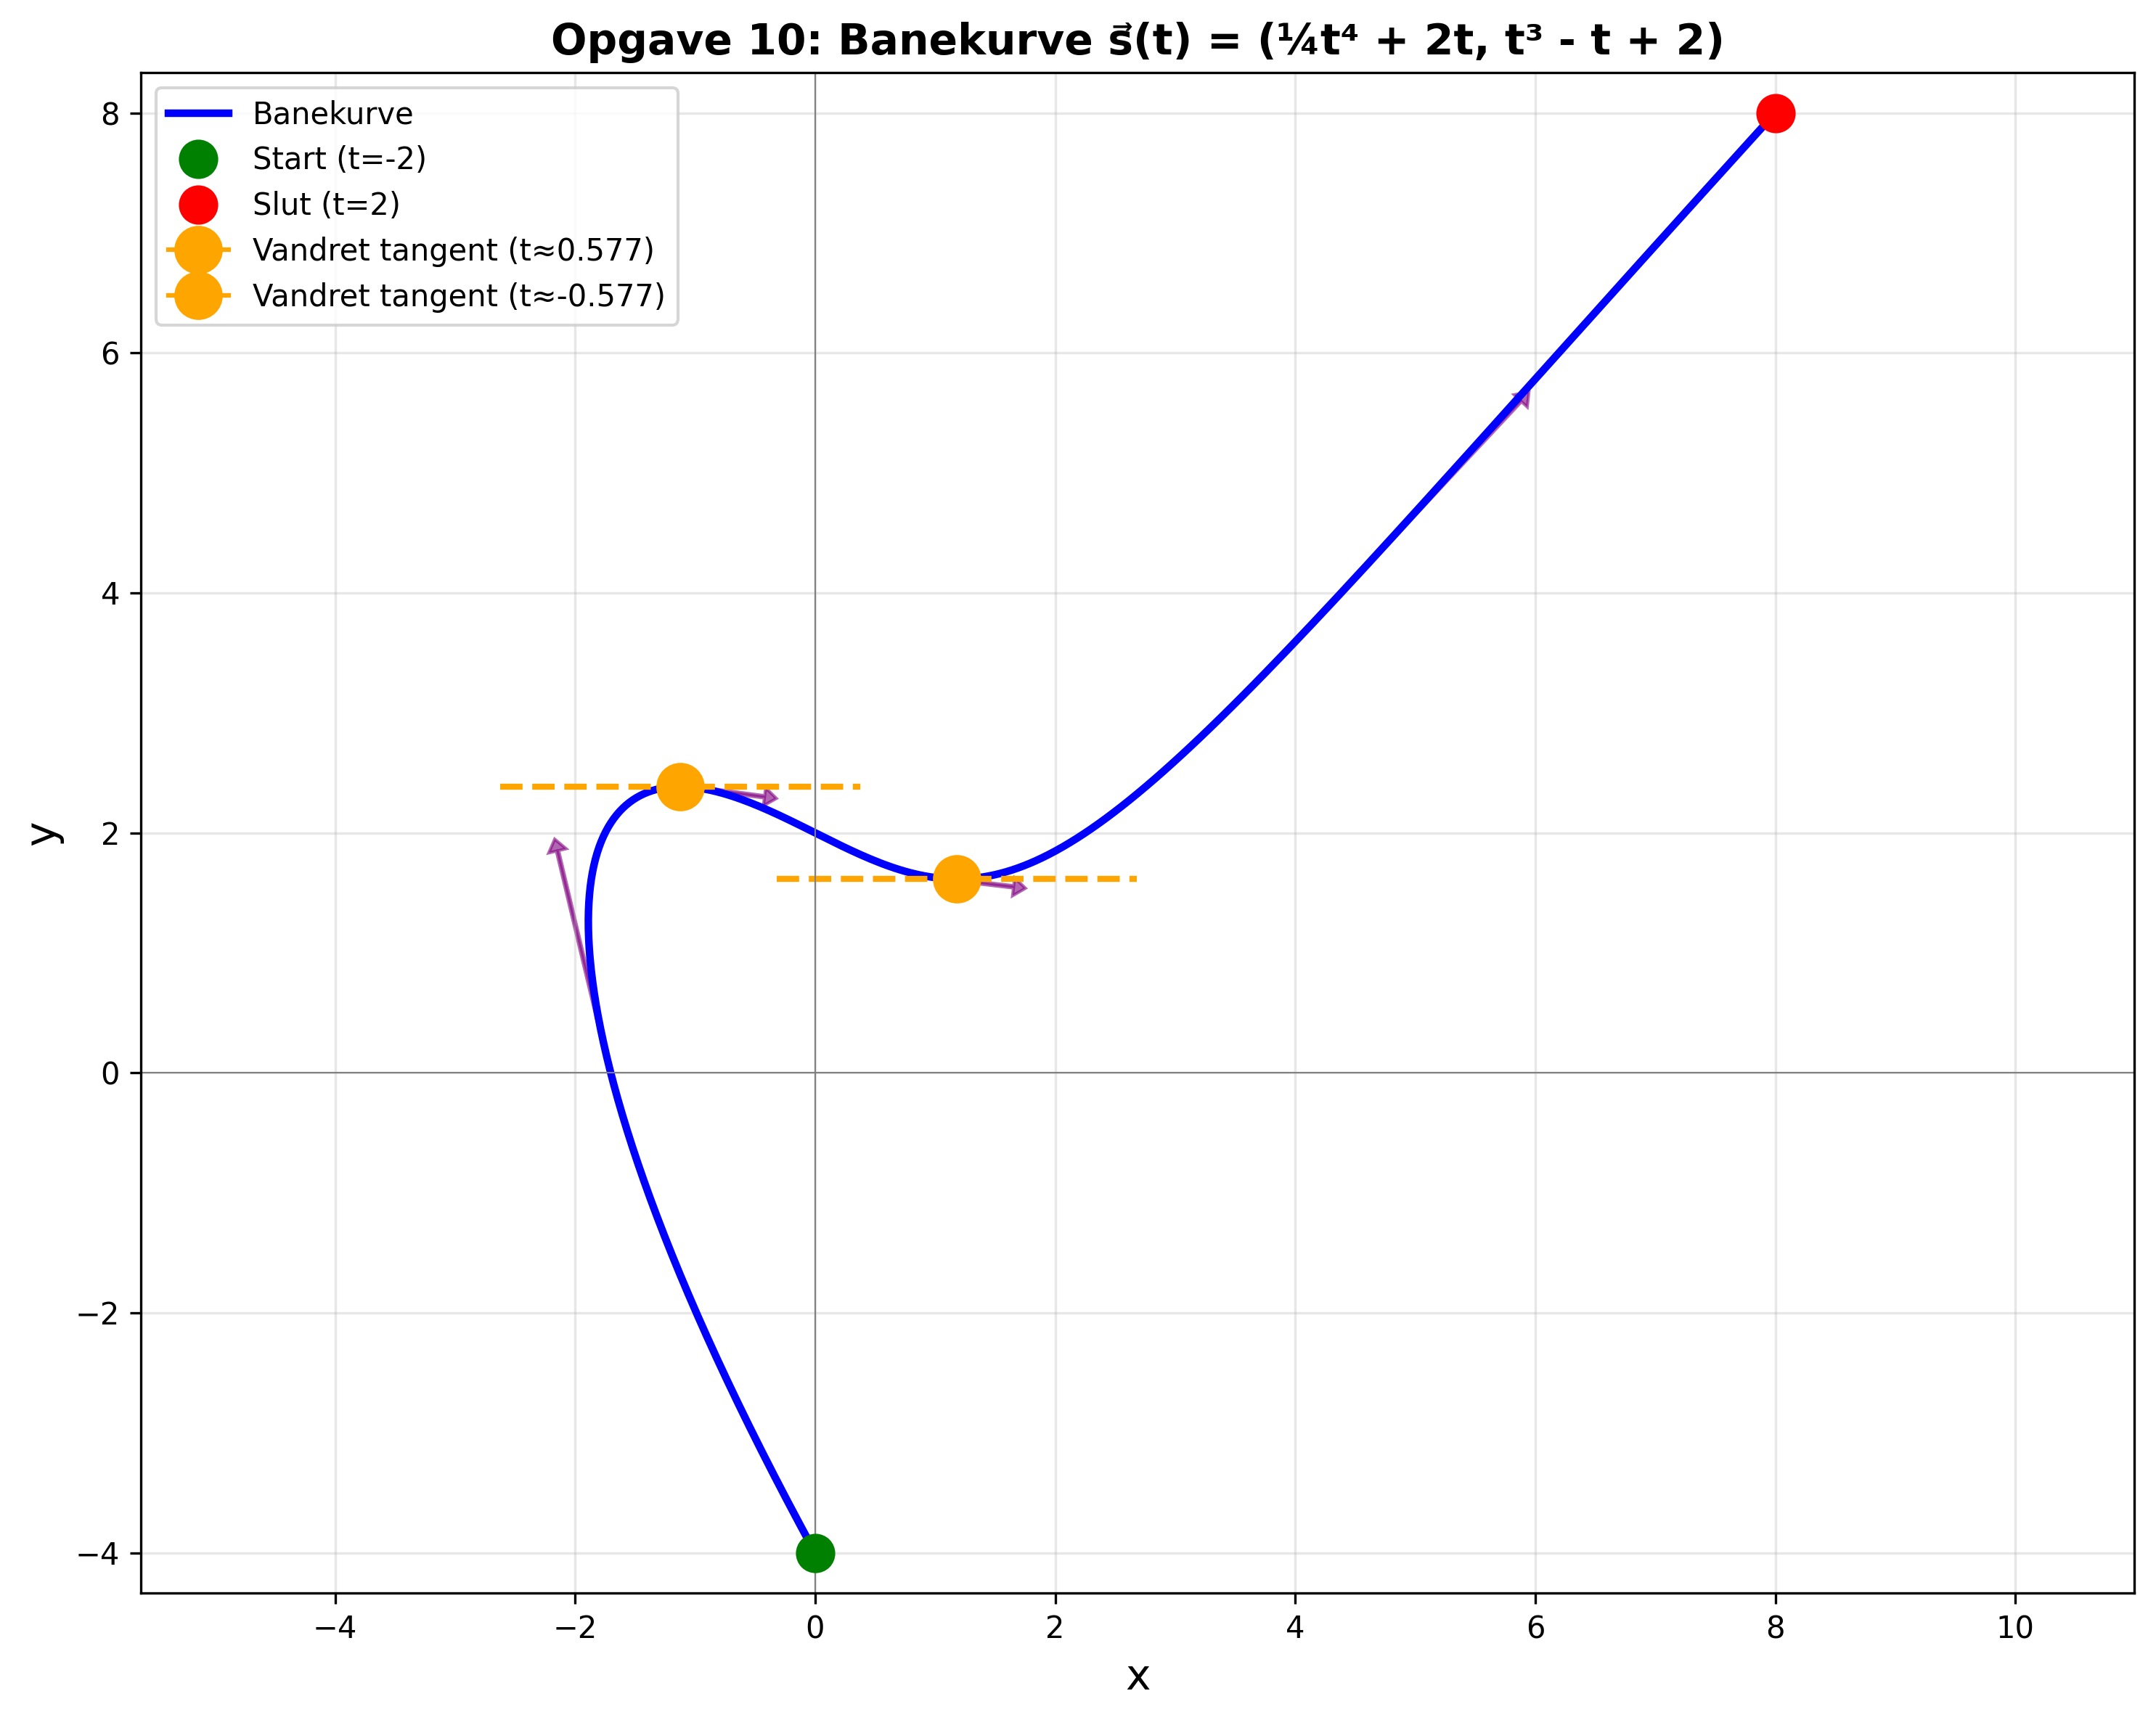
\includegraphics[width=0.95\textwidth]{opgave_10_banekurve.png}
    \caption{Vektorfunktion med vandret tangent ved $t \approx -0.577$ og $t \approx 0.577$}
\end{figure}


\end{document}